% !TeX encoding = ISO-8859-1
\chapter{Solución numérica}
\label{cha:segunda}

 En este capítulo nuestro objetivo es la resolución numérica de la EDP (\ref{ec_1}) mediante el uso de B-spline cuadráticos y el método de Galerkin. Estos conceptos serán introducidos en el marco teórico. Por otro lado, detallaremos el procedimiento realizado para obtener las soluciones numéricas de la EDP (\ref{ec_1}). Por último, realizaremos un análisis de estabilidad del esquema numérico apoyándonos en la teoria de von Neumann.

\section{Marco teórico}

Para hallar la resolución numérica de una EDP, podemos hacerlo utilizando distintas herramientas. En este trabajo utilizaremos el método de Galerkin, basado en el uso de funciones B-spline cuadráticos y funciones peso. En esta sección introduciremos estos conceptos, imprescindibles para el desarrollo.

\subsection{B-spline}

Es bastante común el uso de B-spline, debido a sus buenas características de continuidad y diferenciabilidad entre los nodos. Puede consultar (\cite{prenter9}) para mayor detalle.

\begin{definicion1}[label={definicion},nameref={Title or anything else}]{B-Spline}
    \textit{Dado $m$ valores reales $t_{i}$, denominados nodos, con $t_{0}\leq t_{1} \leq \dots \leq t_{m-1}$ . Se define B-spline de grado $n$ a la curva paramétrica $ S:[t_{0},t_{m-1}] \rightarrow \mathbb R^{2} $ compuesta por una combinación lineal de B-splines básicas $b_{i,n}$ de grado $n$ dado por :}
    $$S(t)=\sum_{i=0}^{m-n-2}P_{i}b_{i,n}(t),$$
    para $t\in [t_{n-1},t_{m-n}]$
\end{definicion1}
Llamamos $P_{i}$ a los puntos de control o puntos de Boor.
Las $m-(n+1)$ B-splines de grado $n$ son funciones a trozos que se pueden definir por construcción de forma recursiva con la fórmula de Cox de Boor.

$$b_{i,n}=\left\{\begin{matrix}
            1 & \text{si} \quad t_{i}\leq t \leq t_{i+1},\\ 
            0 & \text{en otro caso}
\end{matrix}\right.$$
    
    $$b_{i,n}(t)=\frac{t-t_{i}}{t_{i+n}-t_{i}}b_{i,n-1}(t)+\frac{t_{j+n+1}-t}{t_{j+n+1}-t_{j+1}}b_{j+1,n-1}(t).$$

Las funciones definidas B-spline son continuas en los nodos y su derivabilidad dependerá de la distribución de los mismos. Cuando  son equidistantes se dice que son uniformes.

\subsection{Método de Galerkin}

Para realizar la aproximación general de nuestra EDP, continua y con forma bilineal coercitiva vamos a aplicar el Método de Galerkin basado en las funciones peso. En primer lugar, se mostrarán de forma breve aquellos conceptos básicos del análisis funcional necesarios para el desarrollo teórico del método de Galerkin. Para ello, haremos una breve introducción de los espacios de Sobolev.

\subsubsection{Espacios $L^{p}$}

Denotaremos $\Omega$ a un abierto acotado no vacio de $\mathbb R^{d}$, de frontera regular, donde $d \in \mathbb N$. Sea $(\Omega,M,\mu)$ un espacio medible, es decir:

\begin{itemize}
    \item $M$ es un $\sigma$-álgebra en $\Omega$
    \item $\mu$ es medible
    \item $\Omega$ es $\sigma$-finito
\end{itemize}

Definimos $L^{1}(\Omega)$ al espacio de funciones $\Omega$ en $\mathbb R$ que son integrables. En general:

\begin{definicion1}[label={definicion1},nameref={Title or anything else}]{$L^{p}$}
    Sea $p\in \mathbb R$ con $1<p<\infty$.    Definimos:
    \begin{equation}
        L^{p}(\Omega)=\{f:\Omega \longrightarrow \mathbb R: f \ \ es \ \ medible \ \ y \ \ |f|^{p}\in L^{1}(\Omega)\}.
    \end{equation}
    Para todo $f\in L^{p}(\Omega)$, se define $\|f\|_{L^{p}}=\|f\|_{p}=\displaystyle (\int_{\Omega}|f(x)|^{p}d\mu)^{\frac{1}{p}}.$
    
\end{definicion1}

\subsubsection{Espacios de Hilbert}

Sea $H$ un espacio vectorial. Un producto escalar $(u,v)$ es una forma bilineal en $H \times H$ con valores en $\mathbb R$ tal que:

\begin{itemize}
    \item $(u,v)=(v,u), \quad \forall u,v \in H$ (simétrica).
    \item $(u,v)\geq 0, \quad \forall u \in H$ (positiva).
    \item $(u,v) \neq 0, \quad \forall u \neq 0$ (bien definida).
\end{itemize}

El producto escalar satisface la desigualdad de Cauchy-Shwarz:

\begin{equation}
    |(u,v)|\leq (u,u)^{1/2}(v,v)^{1/2}, \quad \forall u,v \in H.
\end{equation}

Como consecuencia tenemos la siguiente norma inducida por el producto escalar:
\begin{equation}
    \|u\|=(u,u)^{1/2}.
\end{equation}
\begin{definicion1}[label={definicion1},nameref={Title or anything else}]{Espacio de Hilbert}
    Definimos espacio de Hilbert a un espacio vectorial $H$ dotado de un producto escalar y tal que $H$ es completo \footnote{Definimos que un espacio es completo cuando todas las sucesiones de Cauchy son convergentes.} para la norma inducida por este producto escalar.
\end{definicion1}


\subsubsection{Espacios de Sobolev}

A continuación, introduciremos brevemente el concepto de derivada débil, los espacios de Sobolev y el Teorema de Lax-Milgram. Para mayor detalle, el lector puede consultar \cite{sobolev4,sobolev6}.


\begin{definicion1}[label={definicion1},nameref={Title or anything else}]{Derivada débil $\partial^{\alpha}u$ }
    \textit{Sea $\Omega \subset \mathbb R^{d}, d \in \mathbb N$. Dado $u,v \in L^{1}(U)$ para $U \subset \mathbb R^{d}$ y $\alpha=(\alpha_{1},\cdots,\alpha_{d})$ es un multi-índice, decimos que $v$ es el $\alpha$-ésima derivada débil de $u$ si y solo si:}
    
    \begin{equation}
        \displaystyle \int_{U} uD^{\alpha}\varphi=(-1)^{|\alpha|}\int_{U}v\varphi.
    \end{equation}
    
    \textit{donde denotamos $\varphi(\Omega)$ al espacio de las funciones de $C^{\infty}(\Omega)$ con soporte compacto en $U$}
    
\end{definicion1}

\begin{definicion1}[label={definicion1},nameref={Title or anything else}]{Espacio de Sobolev}
    \textit{Sea $\Omega \subset \mathbb R^{d},\quad d \in \mathbb N$. Dado $m \in \mathbb N \cup \{0\}$ y $1\leq p \leq +\infty, p \in \mathbb N$ definimos el espacio de Sobolev como:
    \begin{equation}
        W^{m,p}(\Omega):=\{u\in L^{p}(\Omega): \forall \alpha \in \mathbb N^{d} \ con \ |\alpha|\leq m, \partial^{\alpha}u\in L^{p}(\Omega)\}.
    \end{equation}
    donde $\partial^{\alpha}u$ denota, abusando de la notación, la derivada débil de $u$ de orden $|\alpha|$.
    Además, $W^{m,p}_{0}(\Omega)$ se define como la clausura de $C^{\infty}_{0}(\Omega)$ en el espacio $W^{m,p}(\Omega)$}
\end{definicion1}

Podemos observar que $W^{0,p}(\Omega)=L^{p}(\Omega)$ y si $1\leq p < \infty$ entonces $W^{0,p}_{0}(\Omega)=L^{p}(\Omega)$

\begin{teorema1}

\textit{El espacio de Sobolev $W^{m,p}(\Omega)$ es un espacio de Banach}
\end{teorema1}


La norma del espacio de Sobolev se define a partir de la norma $\displaystyle \|\cdot \|_{L^{p}(\Omega )}$

\begin{definicion1}[label={definicion1},nameref={Title or anything else}]{Norma de Sobolev}
    \textit{Sea $u \in W^{m,p}(\Omega)$. Suponemos que la derivada débil $\partial^{\alpha}u$ existe $\forall |\alpha|\leq m$. Definimos la norma de Sobolev como:
    $$\|u\|_{W^{m,p}(\Omega)}:=\big( \sum_{\alpha \leq m}\|\partial^{\alpha}u\|^{p}_{L^{p}(\Omega)})^{\frac{1}{p}},$$ cuando $p<\infty$.\
    Si $p=\infty$ entonces} :
    $$\|u\|_{W^{m,\infty}(\Omega)}:=\max_{\alpha \leq m}\|\partial^{\alpha}u\|_{L^{\infty}(\Omega)}. $$
\end{definicion1}

Denotamos $H^{m}(\Omega):=W^{m,2}(\Omega)$. En consecuencia de lo anterior tenemos entonces:

\begin{proposicion1}

\textit{ El espacio de Sobolev $H^{m}(\Omega)$ es un espacio de Hilbert tal que $\forall u,v \in H^{m}(\Omega)$ el producto escalar es dado por:
$$(u,v)_{H^{m}(\Omega)}:=\sum_{|\alpha|\leq m}(\partial^{\alpha}u,\partial^{\alpha}v)_{L^{2}(\Omega)}.$$
}
\end{proposicion1}

Por tanto, para $p=2$ tenemos que:
\begin{equation}
    \|u\|_{H^{m}(\Omega)}:=(\sum_{|\alpha|\leq m}\|\partial^{\alpha}u\|^{2}_{L^{2}(\Omega)})^{\frac{1}{2}}.
\end{equation}

\begin{definicion1}{$H_{0}^{1}(\Omega)$}
\textit{Definimos el espacio $H_{0}^{1}(\Omega)$ como:
$$H_{0}^{1}(\Omega):=\{u\in H^{1}(\Omega):u|_{\partial(\Omega)}\equiv 0\}.$$
}
\end{definicion1}

Introduciremos una propiedad fundamental en la teoría varicional de las EDP.

\begin{definicion1}{Coercitividad}
\textit{Sea $H$ un espacio de Hilbert y sea $a(\cdot,\cdot):H \times H \longrightarrow \mathbb R$ una forma bilineal definida sobre el espacio $H$. Diremos que la forma bilineal $a(\cdot,\cdot)$ es coercitiva si $\exists \iota>0$ tal que:
$$a(v,v)\geq \iota \|v\|^{2} \quad \forall v\in H$$. 
}
\end{definicion1}

Para poder asegurar la existencia de una solución para la formulación varicional de una EDP vamos a introducir el siguiente resultado:

\begin{teorema1}{Lax-Milgram (Existencia y unicidad)}
\textit{Sea $H$ un espacio de Hilbert, $L(\cdot)$ una forma lineal continua en $H$ y la forma bilineal $a(\cdot,\cdot)$ coercitiva y continua en $H$. Luego para la formulación varicional:
$$a(u,v)=L(v), \quad \forall v\in H,$$ tenemos que existe una única solución $u\in H$ que depende de la forma lineal $L$.
}
\end{teorema1}\label{TH_Lax_M}

Después de introducir brevemente estos conceptos, vamos a proceder a introducir el \textbf{método de Galerkin}.\\

Sea $H$ un espacio de Hilbert, $a(\cdot,\cdot)$ una forma bilineal continua y coercitiva y $L(\cdot)$ lineal y continua definida sobre $H$. Consideramos el problema de formulación varicional de: \begin{equation}\label{problemagalerkin}
    \textit{encontrar $u\in V$ tal que $a(u,v)=L(v) \quad \forall  v\in H$}.
\end{equation}
Este problema variacional se encuentra en las hipótesis del teorema Lax-Milgram \ref{TH_Lax_M}, por lo que existe una única solución $u\in H$ de dicho problema.\\

Aunque se puede ver de forma más general en \cite{galerkin5}, la idea principal del método de Galerkin es encontrar una aproximación de $u\in H$ por un espacio $H_{h}$ de dimensión finita, teniendo la misma norma que la definida en $H$. Para ello vamos a utilizar la aproximación conocida como proyección de Galerkin tomando un subespacio $H_{h}\subseteq H$. Luego introducimos el siguiente problema:
\begin{equation}
\label{praprox}
    \textit{encontrar $u_{h}\in H_{h} \quad \mbox{tal que} \quad a_{h}(u_{h},v_{h})=L(v_{h}) \quad \forall v_{h}\in H_{h}$}
\end{equation}
Este nuevo problema planteado sigue teniendo una única solución $u_{h}\in H_{h} $ puesto que $H_{h}\subseteq H$ y es un espacio de Hilbert \footnote{$H_{h}\subset H$ es un subespacio de un espacio de Banach, por lo que es un subespacio cerrado de un espacio de Hilbert. Por ello, podemos considerar la norma inducida.}. Por lo que se vuelve a cumplir el teorema de Lax-Milgram \ref{TH_Lax_M}.\\

Para proseguir con el método, tenemos que ver que el problema aproximado (\ref{praprox}) es equivalente a un sistema lineal. Puesto que $H_{h}$ es un espacio de dimensión finita, denotamos $N=\dim{H_{h}}$ y $\{\phi _{1},\dots,\phi_{N}\}$ una base de $H_{h}$. Ahora podemos escribir $u_{h}$ como combinación de elementos de la base antes definida:
\begin{equation}
    u_{h}=\displaystyle\sum_{i=1}^{N}U_{i}\phi_{i}
\end{equation}
 donde $U=(U_{i})_{ 1 \leq i \leq N} \in \mathbb R^{N}$, es el vector de coordenadas de $u_{h}$.


\begin{definicion1}{Matriz de rigidez}
Denotamos como matriz de rigidez $A\in \mathbb R^{N \times N}$ definida como:
$$A_{i,j}=a_{h}(\phi_{i},\phi_{j}), 1\leq i,j\leq N$$
\end{definicion1}

Sea $F \in \mathbb R \quad \mbox{y} \quad F_{i}=L(\phi_{i}), \quad 1\leq i \leq N$ podemos escribir nuestro problema entonces como un sistema de ecuaciones lineales de la forma:
\begin{equation}
\label{sistema}
    AU=F
\end{equation}
Llegamos entonces al siguiente resultado:

\begin{proposicion1}
\textit{Sea H un espacio de Hilbert, $a(\cdot , \cdot)$ una forma bilineal continua y coercitiva en $H$ y $L(\cdot)$ forma lineal continua. Si $H_{h}$ es un espacio finito dimensional y se tiene que $H_{h} \subset H$, entonces el problema aproximado (\ref{praprox}) está bien definido y  existe una única solución del sistema (\ref{sistema}).}
\end{proposicion1}

Presentaremos ahora dos resultados que serán útiles para comprobar que la solución del problema (\ref{sistema}) aproxima a la solución del problema (\ref{problemagalerkin}).

\begin{lema1}
      \textit{El error $u-u_{h}$ es a-ortogonal al espacio $H_{h}$}
\end{lema1}

\begin{lema1}
      \textit{Se verifica que}
      \begin{equation}
          \|u-u_{h}\|\leq\frac{M}{\nu}\inf_{v_{h}\in H_{h}}\|u-v_{h}\|,
      \end{equation}
donde $M>0$ y $\nu>0$ son las constantes de continuidad y coercitividad, respectivamente de $a(\cdot,\cdot)$.
\end{lema1}

Este resultado garantiza que si las funciones del espacio $H_{h}$ aproximan a $u$ entonces $u_{h}$ tiende a $u$.

\subsection{Método de Weighted Residuals}

    En matemática aplicada, el método de weighted residual (MWR) es un método para resolver ecuaciones diferenciales. Suponemos que las soluciones de estas ecuaciones diferenciales se aproximan correctamente mediante una suma finita de funciones test $\phi_{i}$. En tales casos, el método MWR se usa para encontrar el valor del coeficiente desconocido de cada función test correspondiente. La solución aproximada se sustituye en la ecuación diferencial gobernante que resulta en un error o residuo. Finalmente, en el MWR el residuo desaparece en los puntos medios o se hace lo más pequeño posible, dependiendo de la función peso, para encontrar los coeficientes desconocidos. Para mayor detalle, consultar \cite{MWR}.\\
    
    Vamos a considerar una EDO,
    \begin{equation}
    \label{ecMWR}
         L(u)=f(x)
    \end{equation}
    sujeto a condiciones de contorno en un dominio $\Omega$. En MWR la solución $u(x)$ de la ecuación (\ref{ecMWR}) es considerada como la aproximación $\hat{u}(x)=\displaystyle\sum_{i=0}^{n}\phi_{i}(x)c_{i}$, que satisface las condiciones de contorno. En este caso, $c_{i}$ son los coeficientes desconocidos aún por determinar, donde $\phi_{i}(x)$ son funciones test linealmente independientes entre sí. La solución asumida se sustituye en la ecuación diferencial gobernante (\ref{ecMWR}), lo que da lugar a un error o residuo. Este residuo es entonces minimizado o forzado a desaparecer en el dominio $\Omega$, dando lugar a un sistema de ecuaciones algebraicas en términos de coeficientes desconocidos $c_{i}$. Como tal, los MWR consisten principalmente en los siguientes pasos:
    
    \begin{itemize}
        \item Primero tomamos la solución aproximada
        \begin{equation}
        \label{ecaproximada}
            u(x)\thickapprox \hat{u}(x)=\displaystyle\sum_{i=0}^{n}\phi_{i}(x)c_{i},
        \end{equation}
        donde $\phi_{i}(x)$ son las funciones test independientes y tal que $\hat{u}(x)$ satisfaga las condiciones de contorno.
        
        \item Sustituimos $\hat{u}(x)$ en la ecuación diferencial $L(\hat{u})-f(x)\neq 0$ el cual da lugar a un error .
        
        \item Definimos el residuo como la medida del error,
        \begin{equation}
        \label{residuo}
            R(x)=L(\hat{u})-f(x).
        \end{equation}
        
        \item Tomamos una función peso $w_{i}(x)$ que será multiplicada a la ecuación (\ref{ecaproximada}) e intregada sobre $\Omega$, obteniendo:
        \begin{equation}
         \displaystyle\int_{\Omega}w_{i}(x)R(x)dx\neq 0,
        \end{equation}
        para $i=0,1,\cdots,n$. Hacer el residuo cero en todo el dominio es de gran dificultad, por lo que pretendemos hacerlo lo mas pequeño posible.
        \item Por último, forzamos que la integral se desvanezca en el dominio $\Omega$:
        \begin{equation}
           \label{MWR0} \displaystyle\int_{\Omega}w_{i}(x)R(x)dx = 0,
        \end{equation}
        obteniendo $n+1$ ecuaciones algebraicas independientes para calcular las incógnitas.
    \end{itemize}
    
    En concreto, en el método de Galerkin consideramos las funciones test como:
    $$w_{k}=\phi_{k}(x) \quad \mbox{para} \quad k=0,1,\ldots,n$$ tal que $\phi_{k}$ sean $n+1$ funciones bases de $x$ que cumplan las condiciones de contorno. Por lo tanto la ecuación (\ref{MWR0}) tendrá la forma:
    \begin{equation}
         \displaystyle\int_{\Omega}\phi_{k}(x)R(x)dx = 0.
    \end{equation}

\section{B-splines cuadrático y propiedades}

Puesto que vamos a aplicar el método de Galerkin, realizamos una discretización en el intervalo $[a,b]$. La discretización en el espacio uniforme viene dada por los nodos $x_{m}$ tales que: $a=x_{0}<x_{1}<\dots<x_{N}=b$ distribuida uniformemente mediante un tamaño de paso $h$ constante: $$h=\frac{b-a}{N}=x_{m+1}-x_{m}.$$

Definimos la siguiente función B-spline cuadrática $\phi_{m}$ siguiendo P.M. Prenter \cite{prenter9}:

\begin{equation}
\label{ec_bspline}
 \phi_{m}(x)=\frac{1}{h^{2}}
        \left\{
        \begin{align}
          (x_{m+2}-x)^{2} -3(x_{m+1}-x)^{2}+3(x_{m}-x)^{2}
          & \quad \text{si} \quad x_{m-1}\leq x \leq x_{m},\\ 
        (x_{m+2}-x)^{2} -3(x_{m+1}-x)^{2} & \quad \text{si} \quad x_{m}\leq x < x_{m+1},\\
        (x_{m+2}-x)^{2} & \quad \text{si} \quad x_{m+1}\leq x < x_{m+2},\\ 
        0 & \quad \quad \text{en otro caso.}
        \end{align}
        \right.
\end{equation} 


\noindent donde los nodos $x_{m}$ están definidos en el intervalo $[a,b]$ para $m=-1(1)N$

El conjunto de funciones $\{\phi_{-1}(x) , \phi_{0}(x) ,\cdots, \phi_{N}(x)\}$  generan una base en el intervalo definido $[a,b]$. Las funciones distintas a $\phi_{m-1} , \phi_{m}$ y $ \phi_{m+1}$ son cero en $[x_{m},x_{m+1}]$. Cada una de estas funciones B-spline cuadráticas abarca tres elementos, por lo que cada $[x_{m},x_{m+1}] $ está cubierta por tres funciones B-spline.\\

\noindent Veamos los valores que toma la función $\phi_{m}(x)$ para los nodos $x_{m-1},x_{m},x_{m+1}$.

\begin{itemize}
    \item $\phi_{m}(x_{m-1})=\frac{1}{h^{2}}[(x_{m+2}-x_{m-1})^{2}-3(x_{m+1}-x_{m-1})^{2}+3(x_{m}-x_{m-1})^{2}]=$\\
    
    $\frac{9h^{2}-12h^{2}+3h^{2}}{h^{2}}=0,$
    
    \item $\phi_{m}(x_{m})=\frac{1}{h^{2}}[(x_{m+2}-x_{m})^{2}-3(x_{m+1}-x_{m})^{2}=\frac{4h^{2}-3h^{2}}{h^{2}}=1,$
    
    \item $\phi_{m}(x_{m+1})=\frac{1}{h^{2}}(x_{m+2}-x_{m+1})^{2}=\frac{h^{2}}{h^{2}}=1.$
    
\end{itemize}


De forma análoga obtendriamos los valores que toma la función $\phi'_{m}(x)$  en los nodos, obteniendo la siguiente Tabla \ref{Tabla}.\\

\begin{table}[h]
\begin{center}
 \begin{tabular}{| c | c | c | c | c |} 
 \hline
    & $x_{m-1}$ & $x_{m}$  & $x_{m+1}$ & $x_{m+2}$ \\ \hline
  $\phi_{m}(x)$ & 0 & 1 & 1 & 0 \\
  $h\phi'_{m}(x)$ & 0 & -2 & 2 & 0 \\ \hline
 \hline
 \end{tabular}
 \end{center}
\end{table}\label{Tabla}

Todas las funciones B-spline diferentes de $\phi_{m-1}(x) , \phi_{m}(x) , \phi_{m+1}(x)$ , son cero sobre el intervalo $[x_{m},x_{m+1}]$.

Una vez definidas estas funciones, definimos la solución numérica dada por:

\begin{equation}
\label{u_n}
    u_{N}(x,t)=\sum_{j=-1}^{N}\phi_{j}(x)\delta_{j}(t),
\end{equation}
 donde $\delta_{j}(t)$ son parámetros dependientes del tiempo que serán determinados por las condiciones de contorno y las condiciones de MWR.\\
 
 Cada intervalo $[x_{m},x_{m+1}]$ finito, puede ser convertido en un intervalo $[0,1]$ aplicando una transformación local de coordenadas definida como:
 \begin{equation}
 \label{CambioVariable}
     h\eta=x-x_{m}, \quad 0\leq \eta \leq 1,
 \end{equation}
De esta manera, puede ser estudiado de forma mas sencilla. Las funciones B-splines cuadráticas (\ref{ec_bspline}) pueden ser definidas en términos de $\eta$ sobre el intervalo $[0,1]$ como:
\begin{equation}\label{CVariablephi}
    \begin{split}
        \phi_{m-1}(\eta) &=(1-\eta)^{2}\\
    \phi_{m}(\eta) &=1+2\eta-2\eta^{2}\\
    \phi_{m+1}(\eta) &=\eta^{2}
    \end{split}
\end{equation}
 La función $u(x,t)$ dada por (\ref{u_n}) sobre $[x_{m},x_{m+1}]$ es aproximada  sobre la región [0,1] por:
$$u_{N}(\eta,t)=\sum_{j=m-1}^{m+1}\phi_{j}\delta_{j}$$ 

Igualando la función (\ref{u_n}) y los B-spline cuadráticos (\ref{ec_bspline}), los valores de $u$ y $u'$ en los nodos son determinados en términos del parámetro $\delta_{m}$ como:
$$u_{N}(x_{m},t)=u_{m}=\delta_{m-1}+\delta_{m}$$
$$u'_{N}(x_{m},t)=u'_{m}=\frac{2}{h}(-\delta_{m-1}+\delta_{m})$$

Dónde el símbolo $``\quad ' \quad "$ denota la primera derivada con respecto a $x$. Los B-spline $\phi_{m}(x)$ y sus primeras derivadas son cero fuera del intervalo $[x_{m-1},x_{m+2}]$

\section{Implementación del método de Galerkin}

Aplicando el método de Galerkin a la ecuación (\ref{ec_1}) tomando como función peso: $w(x)$,  obtenemos la formulación débil de la ecuación:

\begin{equation}
\label{f_pesoNC}
    \int_{a}^{b} w(u_{t}-u_{xxt}-\alpha u_{xx} + \beta u_{x} +uu_{x}) dx =0
\end{equation}

Usando el cambio de variable (\ref{CambioVariable}):

\begin{itemize}
    \item $u_{x}=\frac{\partial u}{\partial x}=\frac{\partial u}{\partial \eta}\frac{\partial \eta}{\partial x}+\frac{\partial u}{\partial t}\frac{\partial t}{\partial x}=\frac{\partial u}{\partial \eta}\frac{\partial \eta}{\partial x}=\frac{1}{h}u_{\eta},$
    \item $u_{xx}=\frac{\partial u_{x}}{\partial x}=\frac{1}{h}\frac{\partial u_{\eta}}{\partial x}=\frac{1}{h}\frac{\partial u_{\eta}}{\partial \eta}\frac{\partial \eta}{\partial x}=\frac{1}{h^{2}}u_{\eta \eta},$
    \item $u_{xxt}=\frac{\partial u_{xx}}{\partial t}=\frac{1}{h^{2}}u_{\eta \eta t}.$
\end{itemize}

Por lo tanto podemos expresar (\ref{f_pesoNC}) como:

\begin{equation}
 \label{f_pesoCV}
    \int_{0}^{1}w(u_{t}-\frac{1}{h^{2}}u_{\eta \eta t}-\frac{\alpha}{h^{2}}u_{\eta \eta}+\frac{\beta}{h}u_{\eta}+\frac{1}{h}\widehat{u}u_{\eta}) d\eta =0
\end{equation}

donde $\widehat{u}$ es tomada como constante local para evitar la no linealidad, facilitando asi también la integral.

Ahora tomando $\rho=\frac{1}{h^{2}}$, $\lambda=\widehat{u}$ y $\xi=\frac{\alpha}{h^{2}}$ y sabiendo que:

\begin{itemize}
    \item $(wu)_{\eta}=w_{\eta}u+wu_{\eta},$
    \item $(wu_{\eta})_{\eta}=w_{\eta}u_{\eta}+wu_{\eta \eta},$
    \item $(wu_{\eta t})_{\eta}=w_{\eta}u_{\eta t}+wu_{\eta \eta t},$
\end{itemize}

tenemos que:

\begin{equation}
\label{ecuacionpartes}
\begin{split}
    \quad w\left(u_{t}-\rho u_{\eta \eta t}-\xi u_{\eta \eta}+\frac{\beta+ \lambda}{h}u_{\eta}\right) & =w\left(u_{t}+\frac{\beta+ \lambda}{h}u_{\eta}\right)-\xi\big(wu_{\eta \eta}-w_{\eta}u_{\eta}\\
    & \quad +w_{\eta}u_{\eta}\big)-\rho wu_{\eta \eta t } \\
    & =
    w\left(u_{t}+\frac{\beta+ \lambda}{h}u_{\eta}\right)-\xi\left((wu_{\eta})_{\eta}+ w_{\eta}u_{\eta}\right)\\
    & \quad -\rho wu_{\eta \eta t }\\ 
    & = w\left(u_{t}+\frac{\beta+ \lambda}{h}u_{\eta}\right)-\xi(\left(wu_{\eta})_{\eta}+ w_{\eta}u_{\eta}\right)\\
    & \quad -\rho( wu_{\eta \eta t } +w_{\eta}u_{\eta t}-w_{\eta}u_{\eta t})\\
    & = w\left(u_{t}+\frac{\beta+\lambda}{h}u_{\eta}\right)-\xi\left(wu_{\eta})_{\eta}+\xi(w_{\eta}u_{\eta}\right)\\
    & \quad +\rho w_{\eta}u_{\eta t} -\rho \left(wu_{\eta t}\right)_{\eta}
\end{split}
\end{equation}


Aplicando la integral por partes en (\ref{f_pesoCV}):

\begin{equation}
\label{13}
    \displaystyle\int_{0}^{1}\left(w(u_{t}+\frac{\beta + \lambda}{h}u_{\eta})+\xi w_{\eta}u_{\eta}+\rho w_{\eta}u_{\eta t} \right) d\eta=\displaystyle\int_{0}^{1}\left(\xi (wu_{\eta})_{\eta}+\rho (wu_{\eta t})_{\eta})\right) d\eta
\end{equation}

Tomando $w(x)$ como las funciones B-splines cuadráticas indicadas en (\ref{ec_bspline}) y sustituyendo la aproximación (\ref{u_n}) en (\ref{13}) con algunas manipulaciones, obtenemos:

$$ \sum_{i,j=m-1}^{m+1}\left[\int_{0}^{1}(\phi_{i}\phi_{j}+\rho\phi'_{i}\phi'_{j})d\eta - \left [\rho \phi_{i}\phi'_{j} \right ]_{0}^{1} \right]\dot{\delta_{j}^{e}}+$$
    
$$ \sum_{i,j=m-1}^{m+1}\left[\int_{0}^{1}(\frac{\beta+\lambda}{h}\phi_{i}\phi'_{j}+\xi\phi'_{i}\phi'_{j})d\eta - \left [\xi \phi_{i}\phi'_{j}\right]_{0}^{1} \right]\delta_{j}^{e}=0,$$

\noindent donde $\delta^{e}=(\delta_{m-1},\delta_{m},\delta_{m+1})^{T}$ y $``\cdot"$ representa la diferenciación respecto a $t$. Puede darse en forma de matriz como:
\begin{equation}
\label{ecABCD_}
    \left[A^{e}+\rho B^{e} - \rho C^{e}\right]\dot{\delta_{j}^{e}}+\left[\frac{\beta + \lambda}{h}D^{e}+\xi B^{e}-\xi C^{e}\right]\delta_{j}^{e}=0.
\end{equation}

\\

Los elementos $a_{ij}^{e}$, $b_{ij}^{e}$, $c_{ij}^{e}$ y $d_{ij}^{e}$ de las matrices $A^{e}, B^{e},C^{e}$ y $ D^{e}$ están dadas por las siguientes integrales:\footnote{Todas las cuentas realizadas para la obtención de las matrices han sido verificadas apoyándome en el software Wolfram Mathematica.}

\begin{equation}
A^{e}_{ij}=\int_{0}^{1}\phi_{i}\phi_{j} d\eta=\frac{1}{30}
\begin{bmatrix}
6 & 13 & 1\\
13 & 54 & 13\\
1 & 13 & 6
\end{bmatrix},
\end{equation}

\begin{equation}
B^{e}_{ij}=\int_{0}^{1}\phi'_{i}\phi'_{j} d\eta=\frac{2}{3}
\begin{bmatrix}
2 & -1 & -1\\
-1 & 2 & -1\\
-1 & -1 & 2
\end{bmatrix},
\end{equation}

\begin{equation}
C^{e}_{ij}=\int_{0}^{1}\phi_{i}\phi'_{j} d\eta=2
\begin{bmatrix}
1 & -1 & 0\\
1 & -2 & 1\\
0 & -1 & 1
\end{bmatrix},
\end{equation}

\begin{equation}
D^{e}_{ij}=\int_{0}^{1}\phi_{i}\phi'_{j}  d\eta=\frac{1}{6}
\begin{bmatrix}
-3 & 2 & 1\\
-8 & 0 & 8\\
-1 & -2 & 3
\end{bmatrix},
\end{equation}\\

\noindent con los subíndices $i,j=m-1 , m , m+1$ para $[x_{m},x_{m+1}]$ . Tomamos $u$ como un promedio (lumped value) de la forma $\frac{u_{m}+u_{m+1}}{2}$ obteniendo:
$$\lambda_{m}=\frac{\delta_{m-1}+2\delta_{m}+\delta_{m+1}}{2}.$$

 Hemos tomado el promedio y lo hemos usado en el siguiente nivel de tiempo como valor aproximado. Debido a esta forma de agrupamiento, se conoce como ``lumped method".\\
 Primero hemos trabajado en el intervalo $[0,1]$ y hemos encontrado $A^{e}, B^{e} , C^{e}$  \mbox{y} $ D^{e}$ para esos elementos. Tenemos entonces que encontrar la solución de la ecuación en todo el intervalo $[a,b]$. Para ello vamos a unir todos los elementos de la matriz en toda la región. Por lo que obtendremos las matrices globales $A, B, C $ y $ D$. Podemos expresar (\ref{ecABCD_}) de forma global como:
\begin{equation}
\label{ecABCDLD}
    \left[ A+\rho B - \rho C \right]\dot{\delta}+\left[ \frac{\beta + \lambda}{h}D+\xi B-\xi C \right]\delta=0
\end{equation}
\noindent donde $\delta=(\delta_{-1},\delta_{0},\delta_{1},\dots,\delta_{N-1},\delta_{N})^{T}$.\\


Veamos el algoritmo utilizado para la obtención de las matrices. Nos centraremos en la matriz $A$\footnote{Todas las cuentas realizadas para la obtención de las matrices han sido verificadas apoyandome en el software Wolfram Mathematica}, las demás matrices se calcularán de forma análoga.\\

Sea $\displaystyle\int_{a}^{b}w(x) u_{t}(x)dx$ y la ecuación (\ref{u_n}). Vamos a fijar los valores de $w$ para obtener las distintas filas de la matriz. Para obtener los coeficientes, vamos a transformar el intervalo $[a,b]$ en el intervalo $[0,1]$ , haciendo uso del cambio de variable (\ref{CambioVariable}),  para facilitar el estudio con el uso de funciones B-splines cuadráticas definidas respecto a $\eta$ (\ref{CVariablephi}).

\begin{itemize}
    \item Para la primera fila de la matriz tomamos: $w(x)=\phi_{-1}(x)$ entonces:

\begin{equation}\label{wphi-1}
    \begin{split}
     \int_{a}^{b}w(x) u_{t}dx & =\int_{a}^{b}\phi_{-1}(x)\sum_{i=-1}^{N}\phi_{i}(x)\delta_{i}(t) dx=\int_{x_{0}}^{x_{1}}\phi_{-1}(x)\sum_{i=-1}^{N}\phi_{i}(x)\delta_{i}(t) dx\\
    & =\int_{x_{0}}^{x_{1}}\phi_{-1}(x)\sum_{i=-1}^{1}\phi_{i}(x)\delta_{i}(t) dx \footnote{Los únicos valores no nulos para este caso son para $i=-1,0,1$}    =\delta_{-1}(t)\int_{x_{0}}^{x_{1}}\phi_{-1}(x)\phi_{-1}(x)dx +\\
    & \quad + \delta_{0}(t)\int_{x_{0}}^{x_{1}}\phi_{-1}(x)\phi_{0}(x)dx + \delta_{1}(t)\int_{x_{0}}^{x_{1}}\phi_{-1}(x)\phi_{1}(x)dx    
    \end{split}
\end{equation}

Procedemos ahora a hacer el cambio de variable. Sea el cambio de variable (\ref{CambioVariable}), las funciones B-splines cuadraticas (\ref{ec_bspline}) y la transfromación al intervalo $[0,1]$ en términos de $\eta$ en  (\ref{CVariablephi}) en el intervalo $[x_{0},x_{1}]$.\\

Para $\phi_{-1}(x)$ en $[x_{0},x_{1}]$:

$$\frac{1}{h^{2}}(x_{1}-x)^{2}=\frac{1}{h^{2}}(x_{1}-x_{0}-h\eta)^{2}=(1-\eta)^{2}=\phi_{m-1}(\eta).$$

Para $\phi_{0}(x)$ en $[x_{0},x_{1}]$:

$$\frac{1}{h^{2}}((x_{2}-x)^{2}-3(x_{1}-x)^{2})=\frac{1}{h^{2}}((x_{2}-x_{0}-h\eta)^{2}-3(h^{2}(1-\eta)^{2}))$$
$$=(2-\eta)^{2}-3((1-\eta)^{2}=1+2\eta-2\eta^{2}=\phi_{m}(\eta).$$

Para $\phi_{1}(x)$ en $[x_{0},x_{1}]$:

$$\frac{1}{h^{2}}((x_{3}-x)^{2}-3(x_{2}-x)^{2}+3(x_{1}-x)^{2})=\frac{1}{h^{2}}((x_{3}-x_{0}-h\eta)^{2}-3(x_{2}-x_{0}-h\eta)^{2}$$
$$+3(x_{1}-x_{0}-h\eta)^{2})=(3-\eta)^{2}-3(2-\eta)^{2}+3(1-\eta)^{2}=\eta^{2}=\phi_{m+1}(\eta).$$

Por lo tanto tenemos que nuestro cambio de variable sería:
\begin{align*}
    \phi_{-1}(x) & \rightarrow \phi_{m-1}(\eta)\\
    \phi_{0}(x) & \rightarrow \phi_{m}(\eta)\\
    \phi_{1}(x) & \rightarrow \phi_{m+1}(\eta)
\end{align*}

Siguiendo entonces (\ref{wphi-1}) y haciendo el cambio anterior para el intervalo $[0,1]$, tenemos que:

\begin{align*}
    \int_{a}^{b}\phi_{-1}(x)u_{t}(x)dx & =\frac{1}{h}\displaystyle \left(\delta_{-1}(t)\int_{0}^{1}\phi_{m-1}(\eta)\phi_{m-1}(\eta)d\eta + \delta_{0}(t)\int_{0}^{1}\phi_{m-1}(\eta)\phi_{m}(\eta)d\eta \\
    & \quad + \delta_{1}(t)\int_{0}^{1}\phi_{m-1}(\eta)\phi_{m+1}(\eta)d\eta )\right  \\
    & = \frac{1}{30h}(6\delta_{-1}(t)+13\delta_{0}(t)+\delta_{1}(t))
\end{align*}
    
Obteniendo así los coeficientes de la primera fila de la matriz $A$.
\end{itemize}

\begin{itemize}
    \item Para la segunda fila de la matriz tomamos $w(x) = \phi_{0}(x)$.\\

Los únicos valores no nulos para $[x_{0},x_{1}]$ son para $i=-1,0,1$ y  $[x_{1},x_{2}]$ son para $i=0,1,2$

\begin{equation}
\label{wphi0}
   \begin{split}
        \int_{a}^{b}w(x) u_{t}(x)dx & =\int_{a}^{b}\phi_{0}(x)\sum_{i=-1}^{N}\phi_{i}(x)\delta_{i(t)}dx=\int_{x_{0}}^{x_{1}}\phi_{0}(x)\sum_{i=-1}^{1}\phi_{i}(x)\delta_{i}dx\\
    & + \int_{x_{1}}^{x_{2}}\phi_{0}(x)\sum_{i=0}^{2}\phi_{i}(x)\delta_{i}(t)=\delta_{-1}(t)\int_{x_{0}}^{x_{1}}\phi_{0}(x)\phi_{-1}(x)dx\\
    & + \delta_{0}(t)\left(\int_{x_{0}}^{x_{1}}\phi_{0}(x)\phi_{0}(x)dx+\int_{x_{1}}^{x_{2}}\phi_{0}(x)\phi_{0}(x)dx\right) \\
    & + \delta_{1}(t)\left(\int_{x_{0}}^{x_{1}}\phi_{0}(x)\phi_{1}(x)dx +\int_{x_{1}}^{x_{2}}\phi_{0}(x)\phi_{1}(x)dx \right)\\
    & +\delta_{2}(t)\int_{x_{1}}^{x_{2}}\phi_{0}(x)\phi_{2}(x)dx.
   \end{split}
\end{equation}


Procedemos ahora a hacer el cambio de variable de forma análoga a la anterior utilizando  \ref{ec_bspline}, \ref{CambioVariable}, y \ref{CVariablephi} en el intervalo $[x_{0},x_{1}]$ y $[x_{1},x_{2}]$ obteniendo los siguientes cambios de variable:\\

Para el intervalo $[x_{0},x_{1}]$:

\begin{align*}
    \phi_{-1}(x) & \rightarrow \phi_{m-1}(\eta)\\
    \phi_{0}(x) & \rightarrow \phi_{m}(\eta)\\
    \phi_{1}(x) & \rightarrow \phi_{m+1}(\eta)
\end{align*}

Para el intervalo $[x_{1},x_{2}]$:

\begin{align*}
    \phi_{0}(x) &\rightarrow \phi_{m-1}(\eta)\\
    \phi_{1}(x) &\rightarrow \phi_{m}(\eta)\\
    \phi_{2}(x) &\rightarrow \phi_{m+1}(\eta)
\end{align*}

Siguiendo entonces (\ref{wphi0}):

\begin{align*}
    (\ref{wphi0}) & =\frac{1}{h} \left[\delta_{-1}\int_{0}^{1}\phi_{m}(\eta)\phi_{m-1}(\eta)d\eta+\delta_{0}\left(\int_{0}^{1}\phi_{m}(\eta)\phi_{m}(\eta)d\eta+\int_{0}^{1}\phi_{m-1}(\eta)\phi_{m-1}(\eta)d\eta\right)\\
    & +\delta_{1}\left(\int_{0}^{1}\phi_{m}(\eta)\phi_{m+1}(\eta)d\eta+\int_{0}^{1}\phi_{m-1}(\eta)\phi_{m}(\eta)d\eta\right)+\delta_{2}\int_{0}^{1}\phi_{m-1}(\eta)\phi_{m+1}(\eta)d\eta\right]\\
    & = \frac{1}{30h}(13\delta_{-1}+60\delta_{0}(t)+26\delta_{1}(t)+\delta_{2}(t)).
\end{align*}
  
Obteniendo así, los coeficientes de la segunda fila.

\end{itemize}

\begin{itemize}
    \item Para las fila del medio tomamos $w(x) = \phi_{j}(x)$ genérico con $j=1,\ldots,N-2$:\\
    
    Los únicos valores no nulos para $[x_{j-1},x_{j}]$ son para $i=j-2,j-1,j$ , para  $[x_{j},x_{j+1}]$ son para $i=j-1,j,j+1$ y $[x_{j+1},x_{j+2}]$ son para $i=j,j+1,j+2$

\begin{equation}
\label{wphim}
\begin{split}
    \int_{a}^{b}w(x) u_{t}(x)dx & =\int_{a}^{b}\phi_{j}(x)\sum_{i=-1}^{N}\phi_{i}(x)\delta_{i}(t) dx=\int_{x_{j-1}}^{x_{j}}\phi_{j}(x)\sum_{i=j-2}^{j}\phi_{i}(x)\delta_{i}(t)dx\\
    & +\int_{x_{j}}^{x_{j+1}}\phi_{j}(x)\sum_{i=j-1}^{j+1}\phi_{i}(x)\delta_{i}(t)+\int_{x_{j+1}}^{x_{j+2}}\phi_{j}(x)\sum_{i=j}^{j+2}\phi_{i}(x)\delta_{i}(t) \\
    & =\delta_{j-2}(t)\int_{x_{j-1}}^{x_{j}}\phi_{j}(x)\phi_{j-2}(x)dx + \delta_{j-1}(t)\Bigg(\int_{x_{j-1}}^{x_{j}}\phi_{j}(x)\phi_{j-1}(x)dx\\
    & +\int_{x_{j}}^{x_{j+1}}\phi_{j}(x)\phi_{j-1}(x)dx\Bigg)+\delta_{j}(t)\Bigg(\int_{x_{j-1}}^{x_{j}}\phi_{j}(x)\phi_{j}(x)dx\\
    & +\int_{x_{j}}^{x_{j+1}}\phi_{j}(x)\phi_{j}(x)dx+\int_{x_{j+1}}^{x_{j+2}}\phi_{j}(x)\phi_{j}(x)dx\Bigg)\\
    & +\delta_{j+1}(t)\Bigg(\int_{x_{j}}^{x_{j+1}}\phi_{j}(x)\phi_{j+1}(x)dx+\int_{x_{j+1}}^{x_{j+2}}\phi_{j}(x)\phi_{j+1}(x)dx\Bigg)\\
    & + \delta_{j+2}(t)\int_{x_{j+1}}^{x_{j+2}}\phi_{j}(x)\phi_{j+2}(x)dx.
    \end{split}
\end{equation}

Procedemos ahora a hacer el cambio de variable de forma análoga a la anterior utilizando \ref{CambioVariable}, \ref{ec_bspline} y \ref{CVariablephi} en el intervalo $[x_{j-1},x_{j}]$ , $[x_{j},x_{j+1}]$ y $[x_{j+1},x_{j+2}]$  obteniendo los siguientes cambios de variable:\\

Para el intervalo $[x_{j-1},x_{j}]$:
\begin{align*}
    \phi_{j-2}(x) & \rightarrow \phi_{m-1}(\eta)\\
    \phi_{j-1}(x) & \rightarrow \phi_{m}(\eta) \\
    \phi_{j}(x) & \rightarrow \phi_{m+1}(\eta)\\
\end{align*}


Para el intervalo $[x_{j},x_{j+1}]$:

\begin{align*}
   \phi_{j-1}(x) & \rightarrow \phi_{m-1}(\eta)\\
   \phi_{j}(x) & \rightarrow \phi_{m}(\eta)\\
   \phi_{j+1}(x) & \rightarrow \phi_{m+1}(\eta)\\
\end{align*}

Para el intervalo $[x_{j+1},x_{j+2}]$:

\begin{align*}
   \phi_{j}(x) & \rightarrow \phi_{m-1}(\eta)\\
   \phi_{j+1}(x) & \rightarrow \phi_{m}(\eta)\\
   \phi_{j+2}(x) & \rightarrow \phi_{m+1}(\eta)\\
\end{align*}

Sustituyendo en (\ref{wphim}):

\begin{align*}
   & \frac{1}{h}\Bigg[\delta_{j-2}(t)\int_{0}^{1}\phi_{m+1}(\eta)\phi_{m-1}(\eta) d\eta+\delta_{j-1}(t)\Big(\int_{0}^{1}\phi_{m}(\eta)\phi_{m+1}(\eta)d\eta\\
    & +\int_{0}^{1}\phi_{m}(\eta)\phi_{m-1}(\eta)d\eta\Big)+\delta_{j}(t)\Big(\int_{0}^{1}\phi_{m+1}(\eta)\phi_{m+1}(\eta)d\eta+\int_{0}^{1}\phi_{m}(\eta)\phi_{m}(\eta)d\eta\\
    & +\int_{0}^{1}\phi_{m-1}(\eta)\phi_{m-1}(\eta)d\eta\Big)+\delta_{j+1}(t)\Big(\int_{0}^{1}\phi_{m}(\eta)\phi_{m+1}(\eta)d\eta+\int_{0}^{1}\phi_{m}(\eta)\phi_{m-1}(\eta)d\eta\Big)\\
    & +\delta_{j+2}(t)\int_{0}^{1}\phi_{m-1}(\eta)\phi_{m+1}(\eta)d\eta \Bigg]\\
    & = \frac{1}{30h}(\delta_{j-2}(t)+26\delta_{j-1}(t)+66\delta_{j}(t)+26\delta_{j+1}(t)+\delta_{j+2}(t))
\end{align*}
   
   Hemos obtenido por tanto, los coeficientes de las fila intermedias.

\end{itemize}

\begin{itemize}
    \item Para la penúltima fila tomamos $w(x)=\phi_{N-1}(x)$\\
    
    Los únicos valores no nulos para $[x_{N-2},x_{N-1}]$ son para $i=N-3,N-2,N-1$ y para  $[x_{N-1},x_{N}]$ son para $i=N-2,N-1,N$

\begin{equation}
\label{wphiN-1}
\begin{split}
    \int_{a}^{b}w(x)u_{t}(x)dx& =\int_{a}^{b}\phi_{N-1}(x)\sum_{i=-1}^{N}\phi_{i}(x)\delta_{i}(t) dx=\int_{x_{N-2}}^{x_{N-1}}\phi_{N-1}(x)\sum_{i=N-3}^{N-1}\phi_{i}(x)\delta_{i}(t)dx\\
    & +\int_{x_{N-1}}^{x_{N}}\phi_{N-1}(x)\sum_{i=N-2}^{N}\phi_{i}(x)\delta_{i}(t)=\delta_{N-3}(t)\int_{x_{N-2}}^{x_{N-1}}\phi_{N-1}(x)\phi_{N-3}(x)dx\\
    & +\delta_{N-2}(t)\Bigg(\int_{x_{N-2}}^{x_{N-1}}\phi_{N-1}(x)\phi_{N-2}(x)dx+\int_{x_{N-1}}^{x_{N}}\phi_{N-1}(x)\phi_{N-2}(x)dx\Bigg)\\
    & +\delta_{N-1}(t)\Bigg(\int_{x_{N-2}}^{x_{N-1}}\phi_{N-1}(x)\phi_{N-1}(x)dx+\int_{x_{N-1}}^{x_{N}}\phi_{N-1}(x)\phi_{N-1}(x)dx\Bigg)\\
    & +\delta_{N}(t)\int_{x_{N-1}}^{x_{N}}\phi_{N-1}(x)\phi_{N}(x)dx.
    \end{split}
\end{equation}
    

Procedemos ahora a hacer el cambio de variable de forma análoga a la anterior utilizando (\ref{ec_bspline}), (\ref{CambioVariable})  y (\ref{CVariablephi}) en el intervalo $[x_{N-2},x_{N-1}]$ y $[x_{N-1},x_{N}]$  obteniendo los siguientes cambios de variable:\\

Para el intervalo $[x_{N-2},x_{N-1}]$:

\begin{align*}
    \phi_{N-3}(x) & \rightarrow \phi_{m-1}(\eta)\\
    \phi_{N-2}(x) & \rightarrow \phi_{m}(\eta)\\
    \phi_{N-1}(x) & \rightarrow \phi_{m+1}(\eta)\\
\end{align*}

Para el intervalo $[x_{N-1},x_{N}]$:

\begin{align*}
    \phi_{N-2}(x) & \rightarrow \phi_{m-1}(\eta)\\
    \phi_{N-1}(x) &\rightarrow \phi_{m}(\eta)\\
    \phi_{N}(x) &\rightarrow \phi_{m+1}(\eta)\\
\end{align*}

Sustituyendo en (\ref{wphiN-1}):

\begin{align*}
    &\frac{1}{h}\Bigg[\delta_{N-3}(t)\int_{0}^{1}\phi_{m+1}(\eta)\phi_{m-1}(\eta)d\eta + \delta_{N-2}(t)\Bigg(\int_{0}^{1}\phi_{m}(\eta)\phi_{m+1}(\eta)d\eta\\
    & +\int_{0}^{1}\phi_{m}(\eta)\phi_{m-1}(\eta)d\eta\Bigg)+\delta_{N-1}(t)\Bigg(\int_{0}^{1}\phi_{m+1}(\eta)\phi_{m+1}(\eta)d\eta\\
    &+\int_{0}^{1}\phi_{m}(\eta)\phi_{m}(\eta)d\eta\Bigg) +\delta_{N}(t)\int_{0}^{1}\phi_{m}(\eta)\phi_{m+1}(\eta)d\eta\Bigg]\\
    & =\dfrac{1}{30h}(\delta_{N-3}(t)+26\delta_{N-2}(t)+60\delta_{N-1}(t)+13\delta_{N}(t)).
\end{align*}

Luego hemos obtenido los coeficientes de la penúltima fila.

\end{itemize}

\begin{itemize}
    \item Por último, tomamos $w(x)=\phi_{N}(x)$\\
    
    Los únicos valores no nulos para $[x_{N-1},x_{N}]$ son para $i=N-2,N-1,N$

\begin{equation}
\label{wphiN}
\begin{split}
    \int_{a}^{b}w(x)u_{t}(x)dx & =\int_{a}^{b}\phi_{N}(x)\sum_{i=-1}^{N}\phi_{i}(x)\delta_{i}(t)dx =\int_{x_{N-1}}^{x_{N}}\phi_{N}(x)\sum_{i=N-2}^{N}\phi_{i}(x)\delta_{i}(t)dx\\
    & =\delta_{N-2}(t)\int_{x_{N-1}}^{x_{N}}\phi_{N}(x)\phi_{N-2}(x)dx +\delta_{N-1}(t)\int_{x_{N-1}}^{x_{N}}\phi_{N}(x)\phi_{N-1}(x)dx\\
    & +\delta_{N}(t)\int_{x_{N-1}}^{x_{N}}\phi_{N}(x)\phi_{N}(x)dx.
    \end{split}
\end{equation}

Procedemos ahora a hacer el cambio de variable de forma análoga a la anterior utilizando \ref{ec_bspline}. \ref{CambioVariable} y \ref{CVariablephi} en el intervalo $[x_{N-1},x_{N}]$ obteniendo los siguientes cambios de variable:\\

Para el intervalo $[x_{N-1},x_{N}]$:


\begin{align*}
    \phi_{N-2}(x) & \rightarrow \phi_{m-1}(\eta)\\
    \phi_{N-1}(x) &\rightarrow \phi_{m}(\eta)\\
    \phi_{N}(x) &\rightarrow \phi_{m+1}(\eta)\\
\end{align*}

Sustituyendo en (\ref{wphiN}):

\begin{align*}
   &\frac{1}{h}\Bigg[\delta_{N-2}(t)\int_{0}^{1}\phi_{m+1}(\eta)\phi_{m-1}(\eta)d\eta + \delta_{N-1}(t)\int_{0}^{1}\phi_{m}(\eta)\phi_{m+1}(\eta)d\eta\\
    & +\delta_{N}(t)\int_{0}^{1}\phi_{m-1}(\eta)\phi_{m-1}(\eta)d\eta\Bigg]=\dfrac{1}{30h}(\delta_{N-2}(t)+13\delta_{N-1}(t)+6\delta_{N}(t)).
\end{align*}
  
  Hemos calculado por tanto los coeficientes de la matriz $A$ completa.
  
\end{itemize}

Las matrices $B, C $ y $ D$ se calculan de forma análoga. Basándonos en el anterior algoritmo y apoyando los cálculos en  Wolfram Mathematica obtenemos las siguientes matrices:

\begin{equation}
\label{a}
    30A=\begin{pmatrix}
         6 & 13 & 1 & 0 & 0 & \cdots & 0\\
         13 & 60 & 26 & 1 & 0 &  \cdots & 0\\
         1 & 26 & 66 & 26 & 1 &  \cdots & 0\\
         0 & \ddots & \ddots & \ddots & \ddots &\ddots & 0\\
         0 & 0 & \cdots & 1 & 26 & 60 & 13 \\
         0 & 0 & \cdots & 0 & 1 & 13 & 6 
         \end{pmatrix}
\end{equation}

\begin{equation}
\label{B}
    \frac{3}{2}B=\begin{pmatrix}
         2 & -1 & -1 & 0 & 0 & \cdots & 0\\
        -1 & 4 & -2 & -1 & 0 &  \cdots & 0\\
        -1 & -2 & 6 & -2 & -1 &  \cdots & 0\\
         0 & \ddots & \ddots & \ddots & \ddots &\ddots & 0\\
         0 & 0 & \cdots & -1 & -2 & 4 & -1 \\
         0 & 0 & \cdots & 0 & -1 & -1 & 2 
         \end{pmatrix}
\end{equation}
    
\begin{equation}
\label{c}
    \frac{1}{2}C=\begin{pmatrix}
         1 & -1 & 0 & 0 & 0 & \cdots & 0\\
         1 & -1 & 0 & 0 & 0 &  \cdots & 0\\
         0 & 0 & 0 & 0 & 0 &  \cdots & 0\\
         0 & \ddots & \ddots & \ddots & \ddots &\ddots & 0\\
         0 & 0 & \cdots & 0 & 0 & -1 & 1 \\
         0 & 0 & \cdots & 0 & 0 & -1 & 1 
         \end{pmatrix}
\end{equation}
    
   \begin{equation}
   \label{D}
    6D=\small{\begin{pmatrix}
        -3\lambda_{0} & 2\lambda_{0} & \lambda_{0} & 0 & 0 & \cdots & 0\\
        -8\lambda_{0} & -3\lambda_{0} & 2\lambda_{0}+ 8\lambda_{1} & \lambda_{0} & 0 &  \cdots & 0\\
        -\lambda_{0} & -2\lambda_{0} - 8\lambda_{1} & 3\lambda_{0}-3\lambda_{2} & 8\lambda_{1}+2\lambda_{2} & \lambda_{2} &  \cdots & 0\\
         0 & \ddots & \ddots & \ddots & \ddots &\ddots & 0\\
         0 & 0 & \cdots & -\lambda_{N-2} & -8\lambda_{N-2}-2\lambda_{N-1} & 3\lambda_{N-2} & 8\lambda_{N-1} \\
         0 & 0 & \cdots & 0 & -\lambda_{N-1} & -2\lambda_{N-1} & 3\lambda_{N-1}
         \end{pmatrix}}
\end{equation}

Donde:
\begin{equation}
    \lambda_{m} & =\frac{1}{2}(\delta_{m-1}+2\delta_{m}+\delta_{m+1})
\end{equation}

Nuestro siguiente objetivo es calcular las funciones $\delta_{j}(t)$.

\subsection{Cálculo de $\delta_{j}(t)$}

Dado que las funciones $\delta_{j}(t)$ dependen de la variable temporal $t$, consideraremos una discretización uniforme en el tiempo tomando $t_{0}<t_{1}<\dots<t_{N}$ con $t_{n+1}-t_{n}=\Delta t$ para $n=0,1,\dots,N_{t}-1$.\\

 A partir de ahora denotaremos cada una de ellas como $\delta_{m}^{n}$, donde la $m$ representa la discretización respecto al espacio y $n$ respecto al tiempo.\\
 
  Vamos a discretizar los $\delta_{i}$ y $\dot{\delta_{i}}$ mediante la aproximación de Crank-Nicolson y una aproximación progresiva en el tiempo, respectivamente.

$$\delta_{i}=\frac{\delta_{i}^{n}+\delta_{i}^{n+1}}{2}, \quad \dot{\delta_{i}}=\frac{\delta_{i}^{n+1}-\delta_{i}^{n}}{\Delta t}$$

Sustituyendo las aproximaciones anteriores en (\ref{ecABCDLD}):

$$[A+\rho B - \rho C]\frac{\delta_{i}^{n+1}-\delta_{i}^{n}}{\Delta t}+(\frac{\beta+\lambda}{h}D+\xi B-\xi C)\frac{\delta_{i}^{n}+\delta_{i}^{n+1}}{2}=0.$$
\begin{equation}
\label{C-N}
    \delta^{n+1}_{i}[A+\rho B - \rho C+(\frac{\beta+\lambda}{h}D+\xi B -\xi C)\frac{\Delta t}{2}]=\delta^{n}_{i}[A+\rho B - \rho C-(\frac{\beta+\lambda}{h}D+\xi B - \xi C)\frac{\Delta t}{2}]
\end{equation}

\noindent con $i=m-2,m-1,m,m+1,m+2$

Este sistema tiene $(N+2)$ ecuaciones lineales con $(N+2)$ coeficientes desconocidos $(\delta_{-1},\delta_{0},\dots,\delta_{N-1},\delta_{N})$. 
Obteniendo un sistema $(N+2)\times (N+2)$ donde $\Delta t$ es el paso del tiempo.

Tomando (\ref{C-N}) y las matrices (\ref{a})-(\ref{D}) obtenemos una relación entre los parámetros $\delta_{i}^{n+1}$ y $\delta_{i}^{n}$ en los niveles de tiempo $n$ y $n+1$ dada por:

\begin{equation}
\label{gammaec}
   \small{\gamma_{1}\delta_{m-2}^{n+1}+\gamma_{2}\delta_{m-1}^{n+1}+\gamma_{3}\delta_{m}^{n+1}+\gamma_{4}\delta_{m+1}^{n+1}+\gamma_{5}\delta_{m+2}^{n+1}=\\
   \centering
   \gamma_{5}\delta_{m-2}^{n}+\gamma_{4}\delta_{m-1}^{n}+\gamma_{3}\delta_{m}^{n}+\gamma_{2}\delta_{m+1}^{n}+\gamma_{1}\delta_{m+2}^{n}}
\end{equation}


\noindent donde los coeficientes $\gamma_{j}$ son:
\begin{align*}
   \gamma_{1} &=\frac{1}{30}-\frac{2\rho}{3}-\frac{\xi \Delta t}{3}-\frac{(\beta+\lambda)\Delta t}{12h}\\
    \gamma_{2} &=\frac{26}{30}-\frac{4\rho}{3}-\frac{2 \xi \Delta t}{3}-\frac{10(\beta+\lambda)\Delta t}{12h}\\
    \gamma_{3} &=\frac{66}{30}+4\rho+2\xi \Delta t \\
    \gamma_{4} &=\frac{26}{30}-\frac{4\rho}{3}-\frac{2\xi \Delta t}{3}+\frac{10(\beta+\lambda)\Delta t}{12h}\\
    \gamma_{5} &=\frac{1}{30}-\frac{2\rho}{3}-\frac{\xi \Delta t}{3}+\frac{(\beta+\lambda)\Delta t}{12h} 
\end{align*}


El sistema (\ref{gammaec}) puede escribirse de la siguiente forma matricial:
\begin{equation}
\label{PQ}
    P\delta^{n+1}=Q\delta^{n}
\end{equation}
\noindent donde $P$ y $Q$ son matrices pentadiagonales de dimensión $(N+2)\times(N+2)$ y $\displaystyle \delta^{n}=(\delta_{-1}^{n},\delta_{0}^{n},\ldots,\delta_{N-1}^{n},\delta_{N}^{n})^{T}$ es el vector que contiene los $(N+2)$ parámetros desconocidos que queremos calcular en el instante de tiempo $n$. La ecuación (\ref{PQ}) presenta la siguiente forma:
 \begin{equation}\label{Matrizge}
     \small{
     \left(\begin{smallmatrix}
        \gamma_{1} & \gamma_{2} & \gamma_{3} & \gamma_{4} & \gamma_{5} & 0 & \cdots & 0\\
        0 & \gamma_{1} & \gamma_{2} & \gamma_{3} & \gamma_{4} & \gamma_{5} & \ddots & 0\\
        \vdots & \ddots & \ddots & \ddots & \ddots &\ddots & \ddots\\
        0 & 0 & \cdots & \gamma_{1} & \gamma_{2} & \gamma_{3} & \gamma_{4} & \gamma_{5}
    \end{smallmatrix}\right)
    \left(\begin{smallmatrix}
       \delta_{-1}^{n+1} \\
       \delta_{0}^{n+1}\\
        \vdots\\
        \delta_{N}^{n+1}
    \end{smallmatrix}\right) =
       \left(\begin{smallmatrix}
        \gamma_{5} & \gamma_{4} & \gamma_{3} & \gamma_{2} & \gamma_{1} & 0 & \cdots & 0\\
        0 & \gamma_{5} & \gamma_{4} & \gamma_{3} & \gamma_{2} & \gamma_{1} & \ddots & 0\\
        \vdots & \ddots & \ddots & \ddots & \ddots &\ddots & \ddots\\
        0 & 0 & \cdots & \gamma_{5} & \gamma_{4} & \gamma_{3} & \gamma_{2} & \gamma_{1}
    \end{smallmatrix}\right)
    \left(\begin{smallmatrix}
       \delta_{-1}^{n} \\
       \delta_{0}^{n}\\
        \vdots\\
        \delta_{N}^{n}
    \end{smallmatrix}\right)}
    \end{equation}


 
 Para resolver (\ref{PQ}), tomaremos que las matrices $P$ y $Q$ pertenecen al instante $n$ que ya conocemos. Por ello, al calcular las variables en el instante $n+1$, las matrices $P$ y $Q$ serán conocidas y obtendremos un sistema lineal y recursivo, que relaciona los niveles de tiempo $n$ y $n+1$. Por tanto, primero necesitamos calcular el vector inicial $\delta^{0}=(\delta_{-1}^{0},\delta_{0}^{0},\dots,\delta_{N-1}^{0},\delta_{N}^{0})^{T}$
 
 
 \subsubsection{Cálculo de los nodos $\delta_{m}^{0}$}
 
 Para calcular el vector $\delta^{0}=(\delta_{-1}^{0},\delta_{0}^{0},\dots,\delta_{N-1}^{0},\delta_{N}^{0})^{T}$ sustituimos la aproximación sobre el intervalo $[a,b]$ en $t=0$ como sigue:
 
 \begin{equation}
     u_{N}(x,0)=\sum_{m=-1}^{N}\phi_{m}(x)\delta_{m}(0)
 \end{equation}
 
 Podemos escribir la solución como sigue:
 $$u_{N}(x_{m},0)=\phi_{m-2}\delta_{m-2}(0)+\phi_{m-1}\delta_{m-1}(0)+\phi_{m}\delta_{m}(0)+\phi_{m+1}\delta_{m+1}(0)+\phi_{m+2}\delta_{m+2}(0)$$
 
 \noindent donde los valores de los B-splines en los nodos $x_{m}$ se calculan a través de la Tabla \ref{Tabla}\\
 
 
 Para el cálculo del vector utilizaremos la condición inicial y una condición de contorno para obtener las $N+2$ ecuaciones necesarias.
 
 \begin{itemize}
    \item De la condición inicial $u(x,0)=f(x)$ tenemos:
    $$u_{N}(x_{m},0)=\delta_{m-1}^{0}+\delta_{m}^{0}=f(x_{m}),$$ con $m=0,1,2,\dots,N$, luego ya conocemos $N+1$ ecuaciones.
\end{itemize}

\begin{itemize}
    \item De las condiciones de contorno, puesto que solo nos falta una ecuación tomaremos la siguiente:\\
    
         $(u_{N})_{x}(a,0)=0$  tenemos:
         
        $$(u_{N})_{x}(a,0)=u_{N}_{x}(x_{0},0)=\frac{-2}{h}(\delta_{-1}^{0}+\delta_{0}^{0})=0.$$
\end{itemize}

Luego tenemos $N+2$ ecuaciones.\\

 
 Por tanto, haciendo uso de las $N+2$ ecuaciones podemos escribir el siguiente sistema matricial:
 
 \begin{equation}
    \begin{pmatrix}
        -2 & 2 & 0 & 0 & \cdots & 0\\
        1 & 1 & 0 & 0 &  \cdots & 0\\
        0 & \ddots & \ddots & \ddots\\
        0 & 0 & \cdots & 0 & 1 & 1
    \end{pmatrix}
    \begin{pmatrix}
       \delta_{-1}^{0} \\
       \delta_{0}^{0}\\
        \vdots\\
        \delta_{N}^{0}
    \end{pmatrix}
    =
        \begin{pmatrix}
       u'_{N}(x_{0},0) \\
       u_{N}(x_{0},0)\\
        \vdots\\
        u_{N}(x_{N-1},0)\\
        u_{N}(x_{N},0)
    \end{pmatrix}
\end{equation}

Para resolver este sistema nos hemos apoyado en el software Wolfram Mathematica.
 
 \subsubsection{Cálculo de los nodos $\delta^{n}_{m}$}
 
Para la obtención del vector $\delta^{n}=(\delta_{-1}^{n},\delta_{0}^{n},\dots,\delta_{N-1}^{n},\delta_{N}^{n})^{T}$ para $n=1,\cdots,N_{t}$, hemos procedido de la siguiente forma:

\begin{itemize}
    \item En primer lugar, después de haber obtenido $\delta^{0}$, calculamos $\delta^{1}$ mediante el sistema matricial (\ref{Matrizge}) para $n=0$, luego relacionamos $\delta^{0}$ y $\delta^{1}$.

    \item Una vez calculado el vector $\delta^{1}$ resolvemos (\ref{Matrizge}) con $n=1$ relacionando ahora $\delta^{1}$ y $\delta^{2}$, siendo $\delta^{1}$ conocida.

    \item Sucesivamente, calculamos el resto de $\delta^{n}$ de forma análoga, hasta llegar a $\delta^{N_{t}}$.
\end{itemize}
 
\section{Análisis de estabilidad mediante von Neumann}

 Mediante el esquema numérico planteado, a partir de los nodos $(x_{m},t_{n})$ de las discretizaciones, hemos calculado lo valores numéricos $\{\delta_{m}^{n}\}$. En consecuencia, presentarán un error de la forma:
$$\delta_{m}^{n}=\delta_{m_{E}}^{n}+\delta_{m}^{n*}$$ 

siendo $\delta_{m}^{n}$ el valor numérico, $\delta_{m_{E}}^{n}$ el valor exacto y $\delta_{m}^{n*}$ el error de $(x_{m},t_{n})$. Para poder aplicar el análisis de estabilidad, linealizaremos la ecuación (\ref{ec_1}) suponiendo, como en la sección anterior, que $\lambda=\hat{u}$, constante local.

\begin{definicion1}[label={definicion},nameref={Title or anything else}]
    \textit{Un método es numéricamente estable si el error $\delta_{m}^{n*}$ está acotado. En caso contrario, el método es numéricamente inestable.}
\end{definicion1}

Para analizar la estabilidad, tomamos un error tipo onda. Este método se conoce como el método de von Neumann. El hecho de considerar este tipo de error, se debe a que en general, los operadores de diferencia lineales admiten soluciones de tipo onda. Un error tipo onda puede escribirse como:
\begin{equation}
\label{VN}
   \delta_{m}^{n*}=\widehat{\delta^{n}}e^{ijkh} 
\end{equation}
donde $\widehat{\delta^{n}}$ representa la amplitud de la onda en el instante $n$ y $k$ el número de onda. Podemos asumir sin pérdida de generalidad que $x_{j}=jh.$

\begin{itemize}
    \item Sustituyendo (\ref{VN}) en (\ref{gammaec}), tenemos que:
    
    \begin{equation}\label{vnsust}
        \varepsilon_{1}\widehat{\delta^{n+1}}e^{i(j-2)kh}+\varepsilon_{2}\widehat{\delta^{n+1}}e^{i(j-1)kh}+\varepsilon_{3}\widehat{\delta^{n+1}}e^{ijkh}+\varepsilon_{4}\widehat{\delta^{n+1}}e^{i(j+1)kh}+\varepsilon_{5}\widehat{\delta^{n+1}}e^{i(j+2)kh}=\\
        
        \eta_{5}\widehat{\delta^{n}}e^{i(j-2)kh}+\eta_{4}\widehat{\delta^{n}}e^{i(j-1)kh}+\eta_{3}\widehat{\delta^{n}}e^{ijkh}+\eta_{2}\widehat{\delta^{n}}e^{i(j+1)kh}+\eta_{1}\widehat{\delta^{n}}e^{i(j+2)kh}
   \end{equation} 
  
\noindent donde:
\begin{align*}
    \varepsilon_{1}& =1-E-M-K(\beta+\lambda_{m}), & \eta_{1}& =1-E+M-K(\beta+\lambda_{m}),\\
    \varepsilon_{2}&=26-2E-2M-10K(\beta+\lambda_{m}), & \eta_{2} &=26-2E+2M-10K(\beta+\lambda_{m}),\\
    \varepsilon_{3} &=66+6E+6M , & \eta_{3} &=66+6E-6M,\\
    \varepsilon_{4} & =26-2E-2M+10K(\beta+\lambda_{m}), & \eta_{4}& =26-2E+2M+10K(\beta+\lambda_{m}),\\
    \varepsilon_{5} &=1-E-M+K(\beta+\lambda_{m}), & \eta_{5} &=1-E+M+K(\beta+\lambda_{m}),
\end{align*}

\noindent donde

$$E=\frac{20}{h^{2}}, \ \ \ \ \ M=\frac{10\alpha}{h^{2}}, \ \ \ \ \ \ K=\frac{5\Delta t}{2h}.$$

    \item Puesto que se trata de una ecuación en diferencias finitas lineal homogénea de coeficientes constantes de primer orden, su solución es de la forma $\widehat{\delta^{n}}=c\lambda^{n}$ con $c$ constante. Sustituimos en la ecuación anterior (\ref{vnsust}), sacamos factor común $e^{ijkh}$ y despejamos $\lambda$:
    \begin{equation}
    \label{lambdadespejado}
        \lambda=\frac{\varepsilon_{1}e^{-2ikh}+\varepsilon_{2}e^{-ikh}+\varepsilon_{3}+\varepsilon_{4}e^{ikh}+\varepsilon_{5}e^{2ikh}}{\eta_{5}e^{-2ikh}+\eta_{4}e^{-ikh}+\eta_{3}+\eta_{2}e^{ikh}+\eta_{1}e^{2ikh}}.
    \end{equation}
    
    \item Transformamos las exponenciales a trigonométricas mediante el cambio $e^{ikh}=cos(kh)+isen(kh)$:
    
    $$\lambda=\frac{\omega_{1}-i\varpi}{\omega_{2}+i\varpi}$$
    
    donde 
    \begin{align*}
        \omega_{1}&=(2-2E+2M)cos(2kh)+(52-4E+4M)cos(kh)+\eta_{3}\\
        \omega_{2}&=(2-2E-2M)cos(2kh)+(52-4E-4M)cos(kh)+\varepsilon_{3}\\
        \varpi& =20K(\beta + \lambda_{m})sin(kh)+2K(\beta + \lambda_{m})sin(2kh)
    \end{align*}
    \item Estudiamos el módulo de $\lambda$:
    
    $$|\lambda |=\Bigg|\frac{\omega_{1}-i\varpi}{\omega_{2}+i\varpi}\Bigg|\leq 1$$
    
    Cuando:
    $${(66h^{2}+60\alpha\delta t)+(52h^{2}-40\alpha\Delta t)cos(kh)+(h^{2}-20\alpha\Delta t)cos(2kh)}>0$$
\end{itemize}

Por ello, nuestro esquema es condicionalmente estable.

\chapter{Ejemplos y comparaciones}

En este capítulo vamos a considerar dos problema test donde calcularemos las soluciones exactas obtenidas en el Capítulo 3 y las soluciones numéricas obtenidas en el Capitulo 4. Estudiaremos, a través de las normas $L_{2}$ y $L_{\infty}$, la eficiencia y precisión de nuestras soluciones numéricas.\\

Para la obtención de las soluciones nos hemos apoyado en el software Wolfram Mathematica

\section{Ejemplo 1}

Consideramos los siguientes valores de los parámetros en la ecuación (\ref{ec_1}):

\begin{equation}
\label{datosej}
    \alpha=0 , \quad \beta=1 , \quad c=1,03 ,\quad h=0,1 ,\quad \Delta t=0,1\\
    
    \mbox{En el dominio}\quad -40 \leq x \leq 60  , \quad 0\leq t \leq 2 \quad
\end{equation}


Esta ecuación es conocida como la ecuación de Benjamin-Bona-Mahony. Estamos considerando una discretización en el espacio con $N=1000$ puntos y $1001$ subintervalos, y un discretización del tiempo con $N_{t}=20$ subintervalos. Tomamos $u(x,0)=f(x)$ siendo $f(x)$ el solitón obtenido (\ref{SolucionExacta}) en $t=0$.

\begin{figure}
  \centering
    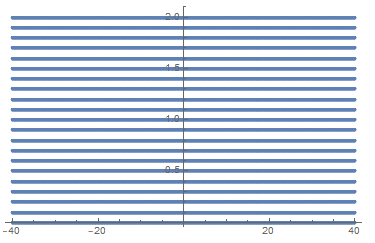
\includegraphics{foto malla.png}
  \caption{Malla para la discretización del intervalo $-40\leq x \leq 60$ tomando $h=0,1$ y $0\leq t \leq 2$ para $\Delta t=0,1$}
  \label{fig:malla}
\end{figure}

\subsection{Solución Exacta}

Tomamos la solución tipo onda solitaria de forma exacta, $u(x,t)$, mediante la expresión obtenida en el Capítulo 3 (\ref{SolucionExacta}). Sustituimos los valores citados anteriormente (\ref{datosej}), obteniendo:

\begin{equation}
    u(x,t)=\frac{9}{100}sech\left[\frac{1}{2}\sqrt{\frac{3}{103}}\left(\frac{-103t}{100}+x\right)\right]^{2}
\end{equation}

Por tanto, la amplitud de onda obtenida es $A=\frac{9}{100}$ y su anchura $\frac{1}{\mu}$ con $\mu=\frac{1}{2}\sqrt{\frac{3}{103}}$

\begin{figure}
  \centering
    \includegraphics{solución exacta.png}
  \caption{Solución exacta del ejemplo}
   \label{fig:SolucionExacta1}
\end{figure} 

Observamos gráficamente la forma del solitón en la Figura \ref{fig:SolucionExacta1}


\subsection{Solución Numérica}

Obtenemos la solución numérica $u_{N}(x,t)$ para este ejemplo, desarrollando el procedimiento descrito en la sección $4.3$ del Capítulo 4. Resolveremos el sistema $(N+2)\times(N+2)$ y hallaremos las $(N+2)$ variables $\{\delta_{m}^{n}\}$.

 \newpage

\subsection{Comparaciones}

En esta sección vamos a comparar ambas soluciones para cada instante de tiempo $n$ aplicando las normas $L_{2}$ y $L_{\infty}$. Para mayor detalle, el lector puede consultar \cite{norma}. Estas normas se definen como:

\begin{equation}
    L_{2}=\|u-u_{N}\|_{2}=\sqrt{h\sum_{m=0}^{N}(u(x_{m},t_{n})-u_{N}(x_{m},t_{n}))^2}
\end{equation}\label{Norma2}

\begin{equation}
    L_{\infty}=\|u-u_{N}\|_{\infty}=\max_{m=0,\ldots,N}|(u(x_{m},t_{n})-(u_{N}(x_{m},t_{n})|
\end{equation}\label{Normainfinito}

\noindent para un $n\in \{0,\ldots,N_{t}\}$ fijado.

Podemos observar la tabla de errores obtenida en \ref{fig:TablaErrores}. Observamos que el error es muy pequeño por lo que podemos concluir que hemos obtenido una solución numérica satisfactoria.

\begin{figure}
  \centering
    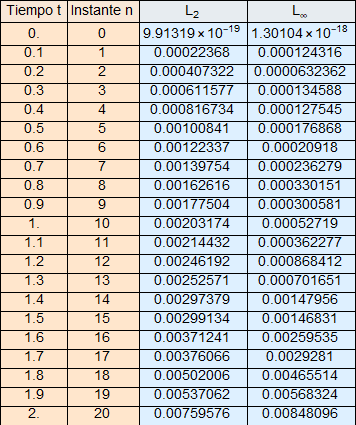
\includegraphics{error nuevo.png}
  \caption{Tabla de errores $L_{2}$ y $L_{\infty}$ entre la solución exacta y la numérica}
  \label{fig:TablaErrores}
\end{figure}

 
\section{Verificación de las leyes de conservación}

Una de las propiedades de las soluciones tipo onda solitaria, en nuestro caso tipo solitón, es la presencia de leyes de conservación. Estas leyes de conservación (masa $M$, momento $P$, energía $E$) vienen dadas por:

\begin{equation}
\label{Masa}
    M=\int_{a}^{b}u(x,t)dx
\end{equation}

\begin{equation}
\label{Momento}
    P=\int_{a}^{b}\bigg(u^{2}(x,t)+u_{x}^{2}(x,t)\bigg)dx
\end{equation}

\begin{equation}
\label{Energia}
    E=\int_{a}^{b}\bigg(u^{3}(x,t)+3u^{2}(x,t)\bigg)dx
\end{equation}

En cada instante de tiempo, vamos a observar en la tabla (\ref{fig:LeyesConservativas}) como las cantidades de masa, momento y energía se mantienen casi constantes con el paso del tiempo. Por lo tanto, se demuestra las buenas propiedades del método numérico.
\begin{figure}[h]
  \centering
    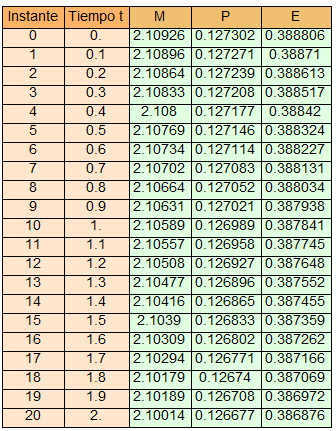
\includegraphics{Leyes conservativas nuevas.png}
  \caption{Leyes de conservación para la solución numérica}
  \label{fig:LeyesConservativas}
\end{figure}
\newpage

\section{Ejemplo 2}

En el anterior ejemplo hemos considerado la condición inicial $u(x,0)$ como el solitón. Podriamos preguntarnos que ocurriría si perturbaramos ligeramente la amplitud del solitón.\\

Vamos a estudiar este caso. Consideramos los mismos valores del ejemplo 1 (\ref{datosej}) para los parámetros en la ecuación (\ref{ec_0y1}). Recordemos que la amplitud de onda obtenida es $A=\frac{9}{100}$.\\

Para la solución numérica, tomamos $u(x,0) = g(x)$ siendo $g(x)$ el solitón obtenido perturbando ligeramente su amplitud. Es decir, vamos a tomar la amplitud de la forma: $\hat{A}= 3(c-1) + 0,05$. Por tanto, sustituyendo los valores (\ref{datosej} ), se define $g(x)$ como:

 \begin{equation}
    g(x)=\frac{14}{100}sech\left[\frac{1}{2}\sqrt{\frac{3}{103}}\left(\frac{-103t}{100}+x\right)\right]^{2}
\end{equation}

Obtenemos la solución numérica $u_{N}(x,t)$ para este ejemplo, desarrollando el procedimiento descrito en el Capítulo 4. Resolveremos el sistema $(N+2)\times(N+2)$ y hallaremos las $(N+2)$ variables $\{\delta_{m}^{n}\}$.

Comprobamos que ocurre con las leyes de conservación. En cada instante de tiempo, observamos en la tabla (\ref{fig:LeyesConservativas1}) como las cantidades de masa, momento y energía se mantienen casi constantes con el paso del tiempo. Por lo que se comporta como un solitón.

\begin{figure}[h]
  \centering
    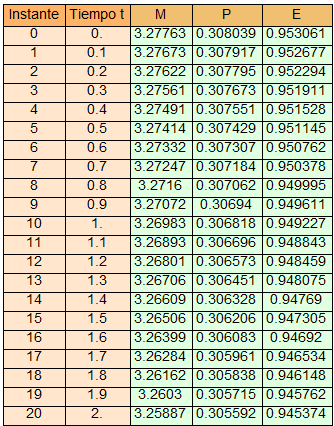
\includegraphics{Leyesconservativas1.png}
  \caption{Leyes de conservación para la solución numérica}
  \label{fig:LeyesConservativas1}
\end{figure}

\chapter{Conclusión}

A través de este trabajo hemos alcanzado satisfactoriamente soluciones tipo solitón de forma exacta y numérica para la ecuación Benjamin-Bona-Mahony-Burger (\ref{ec_1}).\\

Para el cálculo de la solución exacta (\ref{SolucionExacta}) de la ecuación (\ref{ec_0y1}), hemos considerado soluciones tipo onda solitaria obteniendo, por tanto, ondas no lineales estables manteniendo su forma y velocidad sin disiparse en el medio y localizada en un intervalo finito. Hemos realizado un estudio del parámetro $c$, conocido como la velocidad de la onda, además de mostrar gráficamente los diferentes casos.\\

Por otro lado, hemos calculado la solución numérica mediante el método de elementos finitos de Galerkin basado en el uso de funciones B-spline cuadráticos. Hemos podido tomar 1000 puntos para el espacio y 20 para el tiempo. La discretización utilizada ha sido suficiente para calcular soluciones numéricas precisas. Según el análisis de estabilidad realizado mediante la teoria de von Neumann, hemos concluido que el método utilizado es condicionalmente estable. Tanto para la obtención de la solución numérica como para el estudio de la estabilidad, hemos considerado nuestra ecuación de forma linealizada, imponiendo que el término que aportaba la no linealidad, fuera  constante localmente. El estudio de la convergencia se deja para un posible futuro trabajo.\\


Por último, hemos obtenido las soluciones exactas y numéricas de dos problemas test. Hemos comprobado que las soluciones eran prácticamente iguales, obteniendo tablas de errores mediante el uso de las normas $L_{2}$ y $L_{\infty}$. Hemos podido comprobar que la solución numérica ha heredado propiedades de la exacta, como por ejemplo las leyes de conservación. En concreto, hemos probado que nuestras soluciones numéricas mantienen la masa, momento y energía prácticamente constantes a lo largo del tiempo. Por otro lado, hemos realizado un segundo problema test, donde hemos tomado $u(x,t)$ con una pequeña perturbación en la amplitud del solitón.\\

Si se puede, siempre es conveniente hallar la solución exacta, lo que nos ha permitido compararla con la numérica, obteniendo resultados satisfactorios. Concluimos entonces, que el método numérico utilizado es útil y eficaz en nuestra EDP.  \\


Para la realización de todos los cálculos hemos usado el software Wolfram Mathematica, tanto para la implementación del método como para comprobar las cuentas y resultados.

----------------------------------------------------------------------

